\chapter{Analisis}
\label{chap:analisis}


Pada bab ini akan dilakukan analisis mengenai pembangunan simulator pertumbuhan wirausaha dengan \textit{Entrepreneurial Cellular Automata} (ECA). Pembahasan akan dimulai dari analisa pertumbuhan wirausaha di Indonesia yang menjadi pokok permasalahan. Lalu dari analisis ini akan dilanjutkan dengan analisis kebutuhan perangkat lunak agar mampu memodelkan pertumbuhan wirausaha di Indonesia.

% Seorang wirausahawan akan meneruskan usahanya jika nilai CIdx nya memenuhi nilai ambang. Jika nilai dari \textit{Continuity Index} sudah sama atau lebih dari nilai ambang, level wirausaha akan berubah. Sebaliknya, jika nilai dari \textit{Continuity Index }kurang dari sama dengan nilai ambang, level wirausaha bisa saja berubah dan bisa saja tidak berubah.

\section{Analisis Model Pertumbuhan Wirausaha dengan ECA}
\label{analisismodelCA}

Analisis model pertumbuhan wirausaha bergantung terhadap nilai \textit{Continuity Index}, nilai ambang (\textit{threshold}), umur (a) dan usia bisnis (\textit{bl}). Seperti yang sudah dijelaskan pada bab \ref{chap:teori}, \textit{Continuity Index} adalah angka yang menentukan seorang wirausaha akan meneruskan usahanya atau tidak. Sedangkan nilai ambang berfungsi untuk acuan (patokan) perubahan wirausaha dari waktu ke waktu. (Rumus CIDx : \ref{RumusCIDx}).


Untuk mempermudah pemahaman mengenai \textit{Continuity Index}, akan diberikan contoh simulasi dari data tidak real, yaitu terdapat nilai a = 0.5, b = 0.4 dan c = 0.1, nilai ambangnya 15, serta periodenya dalam waktu 5 bulan. Nilai dari faktor psikologis diasumsikan Perceived Opportunities bernilai 0.2, Perceived Capabilities bernilai 0.25, High Status of Successful bernilai 0.1, Public Media Attention bernilai 0.05, Role Model bernilai 0.3 dan Fear of Failure bernilai 0.1. Diasumsikan terdapat tiga wirausahawan dan berikut data dari masing-masing wirausaha :
				
\begin{table} [H]
\centering
\caption{Data wirausahawan}
\begin{tabular}{|c|p{1cm}|p{1cm}|p{1cm}|p{2cm}|p{2cm}|p{2cm}|p{2cm}|p{1cm}|c|}
\hline
& Jenis Kelamin & Umur & Usia Bisnis & Kategori & Sub Kategori & Pendidikan & Lokasi & \textit{Income} & Level\\
\hline
E1 & P & 18th & 0 bulan & Minuman & Minuman bersoda & SMP & Medan & 5-7jt & Nascent\\
\hline
E2 & W & 30th & 0 bulan & Tas & Tas anak-anak  & SMA & Pekanbaru & 3-5jt & New\_bm\\
\hline
E3 & W & 45th & 0 bulan & Makanan & Makanan berat & SD & Palembang & 7-9jt & New\_bm\\
\hline
\end{tabular}
\end{table}

Asumsi ketetanggaan antara wirausaha satu dengan wirausaha lainnya hanya 3 atribut yaitu :

\begin{table} [H]
\centering
\caption{Data Bobot Atribut}
\begin{tabular}{|c|c|}
\hline
Atribut & Bobot\\
\hline
Level Wirausaha & 30\% \\
\hline
Pendidikan & 40\% \\
\hline
Jenis Kelamin & 30\% \\
\hline
\end{tabular}
\end{table}

Masing-masing tetangga relasinya yaitu sama dengan.

	\begin{figure} [H]
		\centering  
		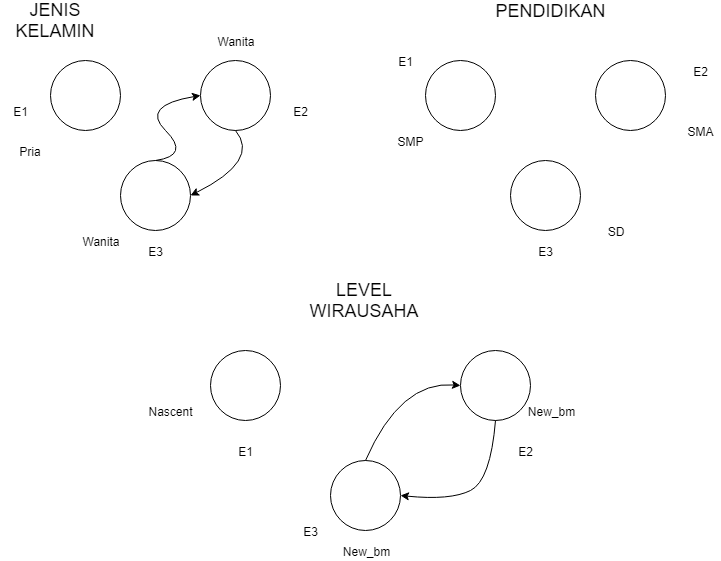
\includegraphics[width=16cm, height=12cm]{t=0} 
		\caption[Gambar ketetanggaan tiga entrepreneur pada saat awal]{Gambar ketetanggaan tiga entrepreneur pada saat awal} 
		\label{fig:t0} 
	\end{figure}


Dalam simulasi ini terdapat 12 faktor publik yang dapat dilihat pada bab \ref{chap:teori} pada tabel \ref{dataPublik}.\\
Berikut rumus CIDx :
\begin{displaymath}
\label{RumusCIDx}
	CIdx_{i}(t) = a.Cint_{i}(t) + b.Cneg_{i}(t) + c.Cpub(t)
\end{displaymath}

Untuk lebih jelasnya berikut contoh perhitungan \textit{continuity index} untuk E2 :
\begin{enumerate}
\item Perhitungan $Cint_{2}(0)$ atau bulan ke 1 :
\begin{enumerate}
	\item Mengambil nilai dari data GEM 2013 sesuai dengan data wirausahawan. Contoh untuk data wirausahawan 1 (E1), terdapat data wanita, 30 tahun, pendidikannya SMA, lokasi di Pekanbaru, pendapatan 3-5 juta rupiah dan level wirausahanya \textit{new\_bm}. Untuk data atribut individual \textit{Perceived Opportunities} nilai untuk wanita 30 tahun adalah 29.5\%, nilai untuk wanita berpendidikan SMA adalah 49.8\%, nilai untuk wanita berlokasi di Pekanbaru adalah 2.8\% dan wanita berpendapatan 3-5juta adalah 41.5\%.
	\item Setelah mendapatkan nilai-nilai dari GEM 2013, nilai-nilai tersebut dijumlahkan lalu dikalikan dengan bobot masing-masing atribut individual. Dalam contoh langkah sebelumnya akan dikalikan dengan 0.2 (\textit{Perceived Opportunities}), berikut penjumlahannya $((29.5+49.8+2.8+41.5) \times 0.2$.
	\item Lakukan langkah pertama dan kedua untuk atribut individual lainnya (\textit{Perceived Capabilities, Role Model, High Status of Successful, Media Attention} dan \textit{Fear of Failure}).
	\item Setelah itu hasil dari masing-masing atribut individual akan dijumlahkan dan dikalikan dengan nilai a (0.5). Berikut perhitungannya :
	\begin{multline}
	CIdx_{2}(t=0) = 0.5 \times (((29.5+49.8+2.8+41.5) \times 0.2) + ((31.6+51.5+2.4+43) \times 0.25) +\\ ((31+41.8) \times 0.3) + ((31+52+2.6+41.7) \times 0.1) + ((3.5+41.6) \times 0.05) + ((32.4+51.7 + 3.8) \times 0.1))
\end{multline}
\end{enumerate}

\item Perhitungan untuk $Cneg_{2}(0)$, kondisi ketetanggaan pada saat awal dapat dilihat pada \ref{fig:t0}. Dapat dilihat bahwa E2 memiliki ketetanggaan berdasarkan jenis kelamin dan level wirausaha dengan E3, sedangkan E2 tidak memiliki ketetanggaan berdasarkan pendidikan maka akan diberi nilai 0. Untuk nilai ketetanggaan berdasarkan jenis kelamin akan diberikan nilai $\frac {1} {2}$, 1 didapat dari jumlah wirausahawan yang bertetanggaan dengan E2 yaitu E3, sedangkan 2 didapat dari total wirausahawan dikurangi 1. Untuk nilai ketetanggaan berdasarkan level wirausaha sama dengan nilai ketetanggaan berdasarkan jenis kelamin. Setelah nilai tersebut didapatkan, nilai tersebut akan dikalikan dengan bobot masing-masing ketetanggaan. Berikut perhitungannya : $(\frac {1} {2} \times 0.3) + 0 +  (\frac {1} {2} \times 0.3)$.

\item Perhitungan pada $Cpub(0)$ :
\begin{enumerate}
	\item Mengalikan nilai-nilai yang ada di tabel \ref{dataPublik} dengan bobot masing-masing faktor publik. Bobot didapatkan dari masukan \textit{user}. Contoh nilai dari faktor publik keuangan terkait dengan kewirausahaan adalah 3.06 lalu dikali dengan bobotnya, sebagai contoh bobotnya 10\%. Maka perkaliannya adalah $3.06 \times 0.1$.
	\item Menjumlahkan hasil perkalian dari langkah pertama. Setelah dijumlahkan hasilnya dibagi dengan banyaknya faktor publik (12) lalu hasilnya dikali dengan nilai c (0.1).\\
	Berikut perhitungannya :
	\begin{multline}
	Cpub(0) = 0.1 \times ((3.06 \times 0.1) + (2.69 \times 0.	1) + (2.22 \times 0.1) + (2.53 \times 0.05) + (2.54 \times 0.1) + (3.3 \times 0.1) \\ + (2.31 \times 0.05) + (3.25 \times 0.05) + (3.92 \times 0.1) + (2.82 \times 0.05) + (3.45 \times 0.1) + (3.29 \times 0.1))\\ = 0.29925 / 12 = 0.0249375 
\end{multline}
\end{enumerate}
\end{enumerate}

Berikut perhitungan CIDx(t=0) :
	\begin{multline}
	CIdx_{1}(t=0) = 0.5 \times (((14.3+4.4+19.9+11) \times 0.2) + ((14.7+17.4+5.4+10.5) \times 0.25) + ((14.3+10.4) \times 0.3) \\ + ((16+19+7.2+10.2) \times 0.1) + ((8.1+11.4) \times 0.05) + ((18.6+18.4+8.9) \times 0.1) ) + 0.4 \times (0 + 0 + 0)\\ + 0.0249375 = 20.09243
\end{multline}
	

\begin{multline}
	CIdx_{2}(t=0) = 0.5 \times (((29.5+49.8+2.8+41.5) \times 0.2) + ((31.6+51.5+2.4+43) \times 0.25) + ((31+41.8) \times 0.3)\\ + ((31+52+2.6+41.7) \times 0.1) + ((3.5+41.6) \times 0.05) + ((32.4+51.7 + 3.8) \times 0.1)) + 0.4 \times ((\frac {1} {2} \times 0.3) + 0 +  (\frac {1} {2} \times 0.3))\\ + 0.0249375 = 51.3749
\end{multline}


\begin{multline}
	CIdx_{3}(t=0) = 0.5 \times (((17.7+17.4+1.4+2.8) \times 0.2) + ((16.1+15.4+3.1+2) \times 0.25) + ((17.6+3) \times 0.3)\\ + ((17+15+5.4+2.2) \times 0.1) + ((5.4+2.7) \times 0.05) + ((16.4+13.9) \times 0.1)) + 0.4 \times ((\frac {1} {2} \times 0.3) + 0 +  (\frac {1} {2} \times 0.3))\\ + 0.0249375 = 15.4374
\end{multline}

	\begin{figure} [H]
		\centering  
		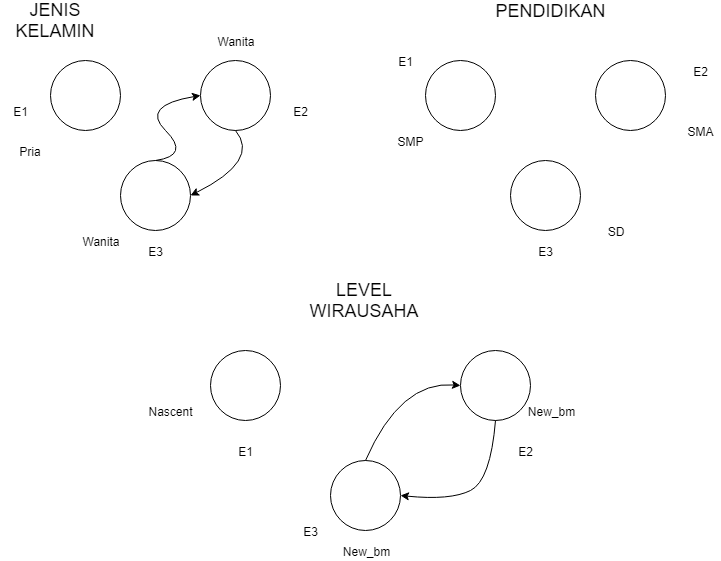
\includegraphics[width=18cm, height=12cm]{t=0} 
		\caption[Gambar ketetanggaan tiga entrepreneur pada saat t = 0]{Gambar ketetanggaan tiga entrepreneur pada saat t = 0} 
		\label{fig:t1} 
	\end{figure}

Perhitungan CIDx (t=1)

\begin{multline}
	CIdx_{1}(t=1) = 0.5 \times (((14.3+4.4+19.9+11) \times 0.2) + ((14.7+17.4+5.4+10.5) \times 0.25) + ((14.3+10.4) \times 0.3) \\ + ((16+19+7.2+10.2) \times 0.1) + ((8.1+11.4) \times 0.05) + ((18.6+18.4+8.9) \times 0.1) ) + 0.4 \times (0 + 0 + 0)\\ +  0.0249375 = 20.09243
\end{multline}

\begin{multline}
	CIdx_{2}(t=1) = 0.5 \times (((29.5+49.8+2.8+41.5) \times 0.2) + ((31.6+51.5+2.4+43) \times 0.25) + ((31+41.8) \times 0.3)\\ + ((31+52+2.6+41.7) \times 0.1) + ((3.5+41.6) \times 0.05) + ((32.4+51.7 + 3.8) \times 0.1)) + 0.4 \times ((\frac {1} {2} \times 0.3) + 0 +  (\frac {1} {2} \times 0.3))\\ +  0.0249375 = 51.3749
\end{multline}

\begin{multline}
	CIdx_{3}(t=1) = 0.5 \times (((17.7+17.4+1.4+2.8) \times 0.2) + ((16.1+15.4+3.1+2) \times 0.25) + ((17.6+3) \times 0.3)\\ + ((17+15+5.4+2.2) \times 0.1) + ((5.4+2.7) \times 0.05) + ((16.4+13.9) \times 0.1)) + 0.4 \times ((\frac {1} {2} \times 0.3) + 0 +  (\frac {1} {2} \times 0.3))\\ +  0.0249375 = 15.4374
\end{multline}

	\begin{figure} [H]
		\centering  
		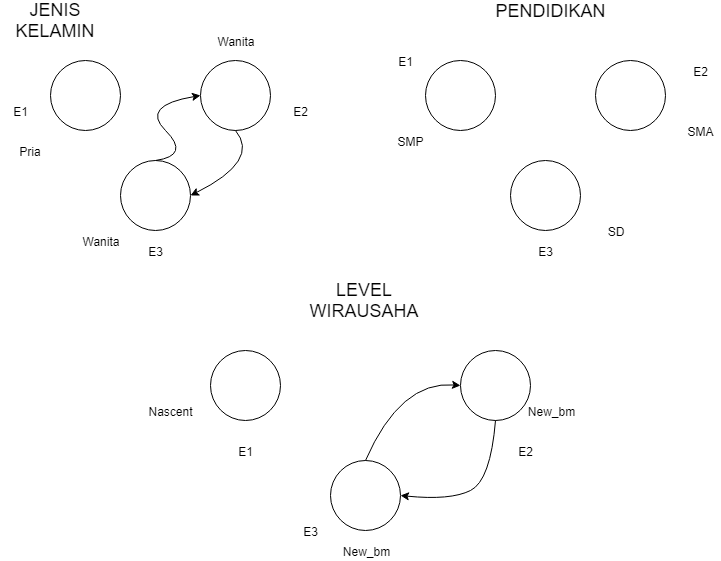
\includegraphics[width=18cm, height=12cm]{t=0} 
		\caption[Gambar ketetanggaan tiga entrepreneur pada saat t = 1]{Gambar ketetanggaan tiga entrepreneur pada saat t = 1} 
		\label{fig:t2} 
	\end{figure}

Perhitungan CIDx (t=2)


\begin{multline}
	CIdx_{1}(t=2) = 0.5 \times (((14.3+4.4+19.9+11) \times 0.2) + ((14.7+17.4+5.4+10.5) \times 0.25) + ((14.3+10.4) \times 0.3) \\ + ((16+19+7.2+10.2) \times 0.1) + ((8.1+11.4) \times 0.05) + ((18.6+18.4+8.9) \times 0.1) ) + 0.4 \times (0 + 0 + 0)\\ +  0.0249375 = 20.09243
\end{multline}

\begin{multline}
	CIdx_{2}(t=2) = 0.5 \times (((29.5+49.8+2.8+41.5) \times 0.2) + ((31.6+51.5+2.4+43) \times 0.25) + ((31+41.8) \times 0.3)\\ + ((31+52+2.6+41.7) \times 0.1) + ((3.5+41.6) \times 0.05) + ((32.4+51.7 + 3.8) \times 0.1)) + 0.4 \times ((\frac {1} {2} \times 0.3) + 0 +  (\frac {1} {2} \times 0.3))\\ +  0.0249375 = 51.3749
\end{multline}

\begin{multline}
	CIdx_{3}(t=2) = 0.5 \times (((17.7+17.4+1.4+2.8) \times 0.2) + ((16.1+15.4+3.1+2) \times 0.25) + ((17.6+3) \times 0.3)\\ + ((17+15+5.4+2.2) \times 0.1) + ((5.4+2.7) \times 0.05) + ((16.4+13.9) \times 0.1)) + 0.4 \times ((\frac {1} {2} \times 0.3) + 0 +  (\frac {1} {2} \times 0.3))\\ +  0.0249375 = 15.4374
\end{multline}

	\begin{figure} [H]
		\centering  
		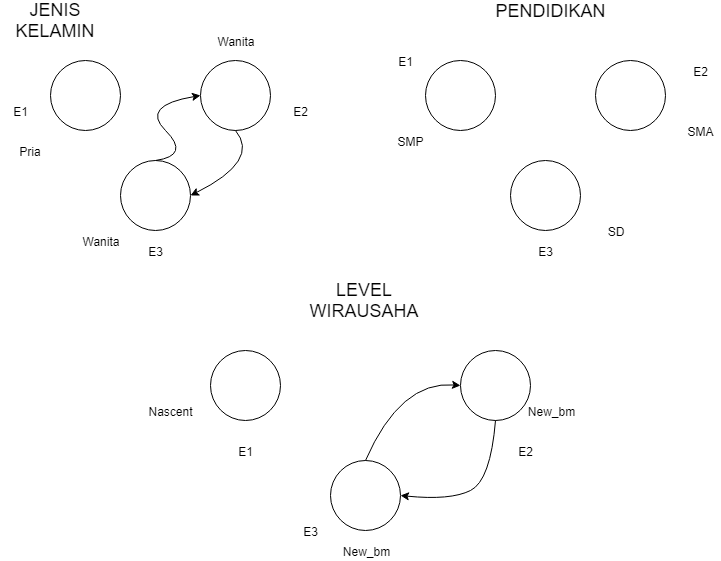
\includegraphics[width=18cm, height=12cm]{t=0} 
		\caption[Gambar ketetanggaan tiga entrepreneur pada saat t = 2]{Gambar ketetanggaan tiga entrepreneur pada saat t = 2} 
		\label{fig:t3} 
	\end{figure}
	
Perhitungan CIDx (t=3)

\begin{multline}
	CIdx_{1}(t=3) = 0.5 \times (((14.3+4.4+19.9+11) \times 0.2) + ((14.7+17.4+5.4+10.5) \times 0.25) + ((14.3+10.4) \times 0.3)\\ + ((16+19+7.2+10.2) \times 0.1) + ((8.1+11.4) \times 0.05) + ((18.6+18.4+8.9) \times 0.1) ) + 0.4 \times (0 + 0 + \frac{2}{2} \times 0.3)\\ +  0.0249375 = 20.2124
\end{multline}

\begin{multline}
	CIdx_{2}(t=3) = 0.5 \times (((29.5+49.8+2.8+41.5) \times 0.2) + ((31.6+51.5+2.4+43) \times 0.25) + ((31+41.8) \times 0.3)\\ + ((31+52+2.6+41.7) \times 0.1) + ((3.5+41.6) \times 0.05) + ((32.4+51.7 + 3.8) \times 0.1)) + 0.4 \times ((\frac {1} {2} \times 0.3) + 0 +  (\frac {2} {2} \times 0.3))\\ +  0.0249375 = 51.4349
\end{multline}

\begin{multline}
	CIdx_{3}(t=3) = 0.5 \times (((17.7+17.4+1.4+2.8) \times 0.2) + ((16.1+15.4+3.1+2) \times 0.25) + ((17.6+3) \times 0.3)\\ + ((17+15+5.4+2.2) \times 0.1) + ((5.4+2.7) \times 0.05) + ((16.4+13.9) \times 0.1)) + 0.4 \times ((\frac {1} {2} \times 0.3) + 0 +  (\frac {2} {2} \times 0.3))\\ +  0.0249375 = 15.4974
\end{multline}

	\begin{figure} [H]
		\centering  
		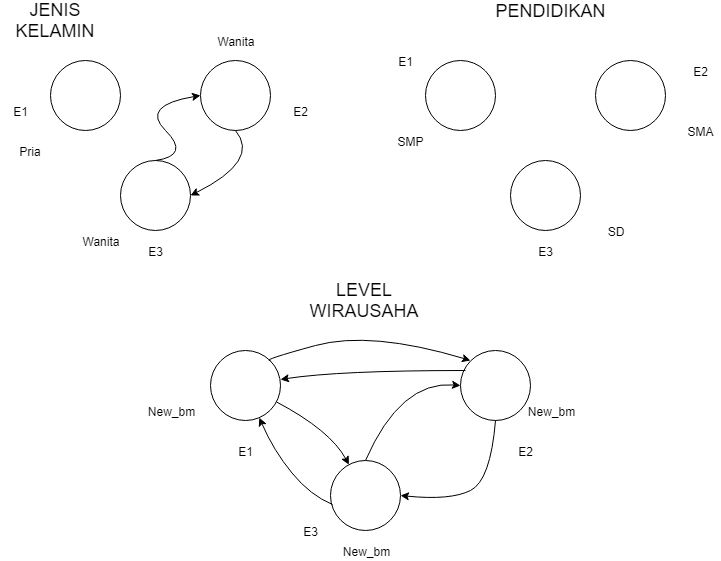
\includegraphics[width=18cm, height=12cm]{t=3} 
		\caption[Gambar ketetanggaan tiga entrepreneur pada saat t = 3]{Gambar ketetanggaan tiga entrepreneur pada saat t = 3} 
		\label{fig:t4} 
	\end{figure}
	
	Perhitungan CIDx (t=4)

\begin{multline}
	CIdx_{1}(t=4) = 0.5 \times (((14.3+4.4+19.9+11) \times 0.2) + ((14.7+17.4+5.4+10.5) \times 0.25) + ((14.3+10.4) \times 0.3)\\ + ((16+19+7.2+10.2) \times 0.1) + ((8.1+11.4) \times 0.05) + ((18.6+18.4+8.9) \times 0.1) ) + 0.4 \times (0 + 0 + \frac{2}{2} \times 0.3)\\ +  0.0249375 = 20.48675
\end{multline}

\begin{multline}
	CIdx_{2}(t=4) = 0.5 \times (((29.5+49.8+2.8+41.5) \times 0.2) + ((31.6+51.5+2.4+43) \times 0.25) + ((31+41.8) \times 0.3)\\ + ((31+52+2.6+41.7) \times 0.1) + ((3.5+41.6) \times 0.05) + ((32.4+51.7 + 3.8) \times 0.1)) + 0.4 \times ((\frac {1} {2} \times 0.3) + 0 +  (\frac {2} {2} \times 0.3))\\ +  0.0249375 = 51.70925
\end{multline}

\begin{multline}
	CIdx_{3}(t=4) = 0.5 \times (((17.7+17.4+1.4+2.8) \times 0.2) + ((16.1+15.4+3.1+2) \times 0.25) + ((17.6+3) \times 0.3)\\ + ((17+15+5.4+2.2) \times 0.1) + ((5.4+2.7) \times 0.05) + ((16.4+13.9) \times 0.1)) + 0.4 \times ((\frac {1} {2} \times 0.3) + 0 +  (\frac {2} {2} \times 0.3))\\ +  0.0249375 = 15.77175
\end{multline}

	\begin{figure} [H]
		\centering  
		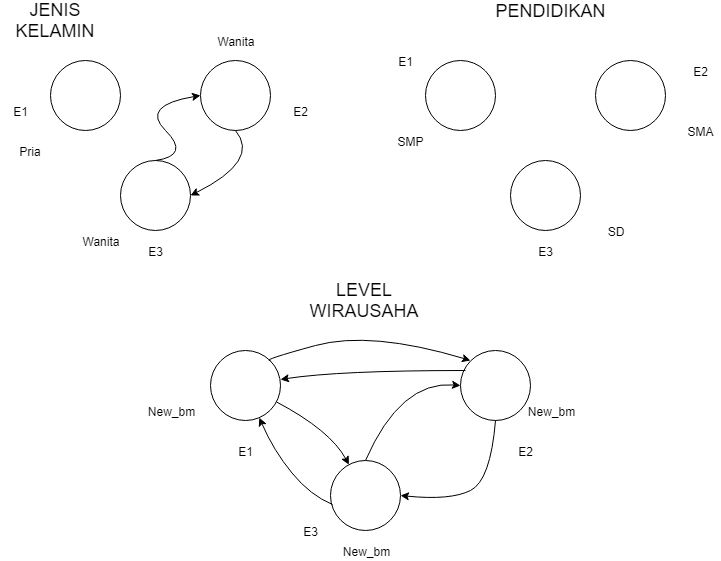
\includegraphics[width=18cm, height=12cm]{t=3} 
		\caption[Gambar ketetanggaan tiga entrepreneur pada saat t = 4]{Gambar ketetanggaan tiga entrepreneur pada saat t = 4} 
		\label{fig:t5} 
	\end{figure}
	
Jadi hasil dari simulasi ini adalah pada bulan pertama wirausaha 1 berada pada level \textit{nascent} dan wirausaha 2 dan 3 berada pada level \textit{new\_bm}. Bulan kedua dan ketiga masih sama, bulan keempat mengalami perubahan pada level wirausaha 1 yaitu dari \textit{nascent} berubah menjadi \textit{new\_bm} sehingga ketiga wirausaha pada bulan keempat berada pada level wirausaha yang sama, begitu juga pada bulan kelima.
	
\section{Deskripsi Perangkat Lunak}
\label{dpl}

Dalam skripsi ini penulis merancang sebuah simulator dari Entrepreneurial Cellular Automata (ECA) yang sebelumnya telah dikembangkan oleh Cecilia Esti Nugraheni dan Vania Natali \cite{ECA}. Simulator ini dinamakan Simulator Pertumbuhan Wirausaha Berbasis Cellular Automata.\\
Perangkat lunak ini dibuat untuk memberi gambaran kepada pemerintah atau lembaga umum mengenai pergerakan wirausaha dalam waktu tertentu. Masukan dari simulator ECA ini yaitu berupa parameter-parameter simulasi yang terdiri dari bobot atribut, relasi antar wirausaha dan nilai a,b,c, \textit{threshold} dan periode. Proses yang dijalankan yaitu pada perhitungan \textit{Continuity Index} yang perhitungannya terbagi menjadi 3 tahap yaitu perhitungan pada faktor internal, perhitungan pada faktor ketetanggaan dan perhitungan pada faktor publik. Hasil keluaran dari simulator ini terdiri dari dua keluaran yaitu keluaran yang ditampilkan pada layar yang berupa jumlah wirausaha pada level tertentu yang ditampilkan per bulan, hasil keluaran kedua yaitu berupa perubahan setiap individu wirausaha dalam setiap bulannya pada \textit{file} CSV yang dapat dibuka pada Microsoft Excel.


\section{Analisis Perangkat Lunak}
\label{analisisPL}

\subsection{Diagram \textit{Use Case}}

Pada diagram \textit{use case} hanya terdapat satu aktor yaitu pemerintah sebagai \textit{user}. Diagram \textit{use case} dapat dilihat pada gambar \ref{fig:usecase}.

	\begin{figure} [H]
		\centering  
		\includegraphics[width=14cm, height=14cm]{usecase1} 
		\caption[Use Case ECA]{Use Case ECA} 
		\label{fig:usecase} 
	\end{figure}
	
Berdasarkan hasil analisis, dibentuk 3 \textit{use case} dengan 1 aktor, yaitu :
\begin{enumerate}
	\item \textbf{Memasukkan parameter simulasi}
	
	\textit{User} dapat memasukkan parameter seperti bobot setiap ketetanggaan, relasi ketetanggaan, bobot faktor publik, mengisi nilai a,b,c dan \textit{threshold} serta periode.
	\item \textbf{Memasukkan file data wirausaha dalam format text}
	
	\textit{User} dapat memasukkan data wirausaha yang akan disimulasikan berupa \textit{file} text.
	\item \textbf{Menjalankan simulasi}
	
	\textit{User} dapat menjalankan simulasi dan melihat hasil simulasi setiap bulannya.
\end{enumerate}

\textbf{Skenario \textit{Use Case}}
\begin{enumerate}
	\item Memasukkan parameter simulasi
	
		\begin{itemize}
			\item Nama : Memasukkan Parameter Simulasi
			\item Aktor : \textit{User}
			\item Deskripsi : Memasukkan bobot untuk setiap atribut dan parameter penting dalam simulasi.
			\item Kondisi awal : \textit{User} belum mengisi bobot untuk setiap atribut dan parameter dalam simulasi.
			\item Kondisi akhir : \textit{User} telah mengisi bobot untuk setiap atribut dan parameter dalam simulasi.
			\item Skenario utama :
		\end{itemize}
		
\begin{table}[H]
\centering
\caption{Tabel Skenario Memasukkan Parameter Simulasi}
\begin{tabular}{|c|p{7cm}|p{7cm}|}
\hline
No & Aksi & Reaksi Sistem\\
\hline
1 & \textit{User} memasukkan parameter simulasi & Sistem akan menyimpan masukan parameter dari \textit{user}.\\
\hline
\end{tabular}
\label{tabelSkenario1}
\end{table}

	\item Memasukkan \textit{File} Data Wirausaha Dalam Format Text
	\begin{itemize}
		\item Nama : Memasukkan \textit{file} data wirausaha dalam format text.
		\item Aktor : \textit{User}.
		\item Deskripsi : Memasukkan \textit{file} data wirausaha yang akan disimulasikan.
		\item Kondisi awal : \textit{User} memasukkan \textit{file} data wirausaha dalam format text.
		\item Kondisi akhir : Sistem akan menampilkan isi data pada tabel.
		\item Skenario utama:
	\end{itemize}
	
	\begin{table}[H]
\centering
\caption{Tabel Skenario Memasukkan \textit{file} data wirausaha dalam format text}
\begin{tabular}{|c|p{7cm}|p{7cm}|}
\hline
No & Aksi & Reaksi Sistem\\
\hline
1 & \textit{User} memilih \textit{file} dan memasukkan \textit{file} data wirausaha dalam format text. & Sistem akan menampilkan isi data pada tabel. \\
\hline
\end{tabular}
\label{tabelSkenario2}
\end{table}

	\item Menjalankan Simulasi
		\begin{itemize}
			\item Nama : Menjalankan Simulasi
			\item Aktor : \textit{User}
			\item Deskripsi : Menjalankan simulasi dan melihat hasil simulasi
			\item Kondisi awal : \textit{User} menjalankan program
			\item Kondisi akhir : Sistem akan menampilkan hasil di tabel dan sistem juga akan mengeluarkan hasil rincian perubahan individu wirausaha pada \textit{file} CSV.
			\item Skenario utama:
		\end{itemize}
		
\begin{table}[H]
\centering
\caption{Tabel Skenario Menjalankan Simulasi}
\begin{tabular}{|c|p{7cm}|p{7cm}|}
\hline
No & Aksi & Reaksi Sistem\\
\hline
1 & \textit{User} menjalankan program & Sistem akan menampilkan hasil di tabel dan sistem juga akan mengeluarkan hasil rincian perubahan individu wirausaha pada \textit{file} CSV \\
\hline
\end{tabular}
\label{tabelSkenario3}
\end{table}
		
\end{enumerate}


\subsection{Diagram Kelas}


Pada bagian ini akan diberikan diagram kelas ECA yang merupakan hasil akhir dari penelitian Nugraheni dan Natali.

	\begin{figure} [H]
		\centering  
		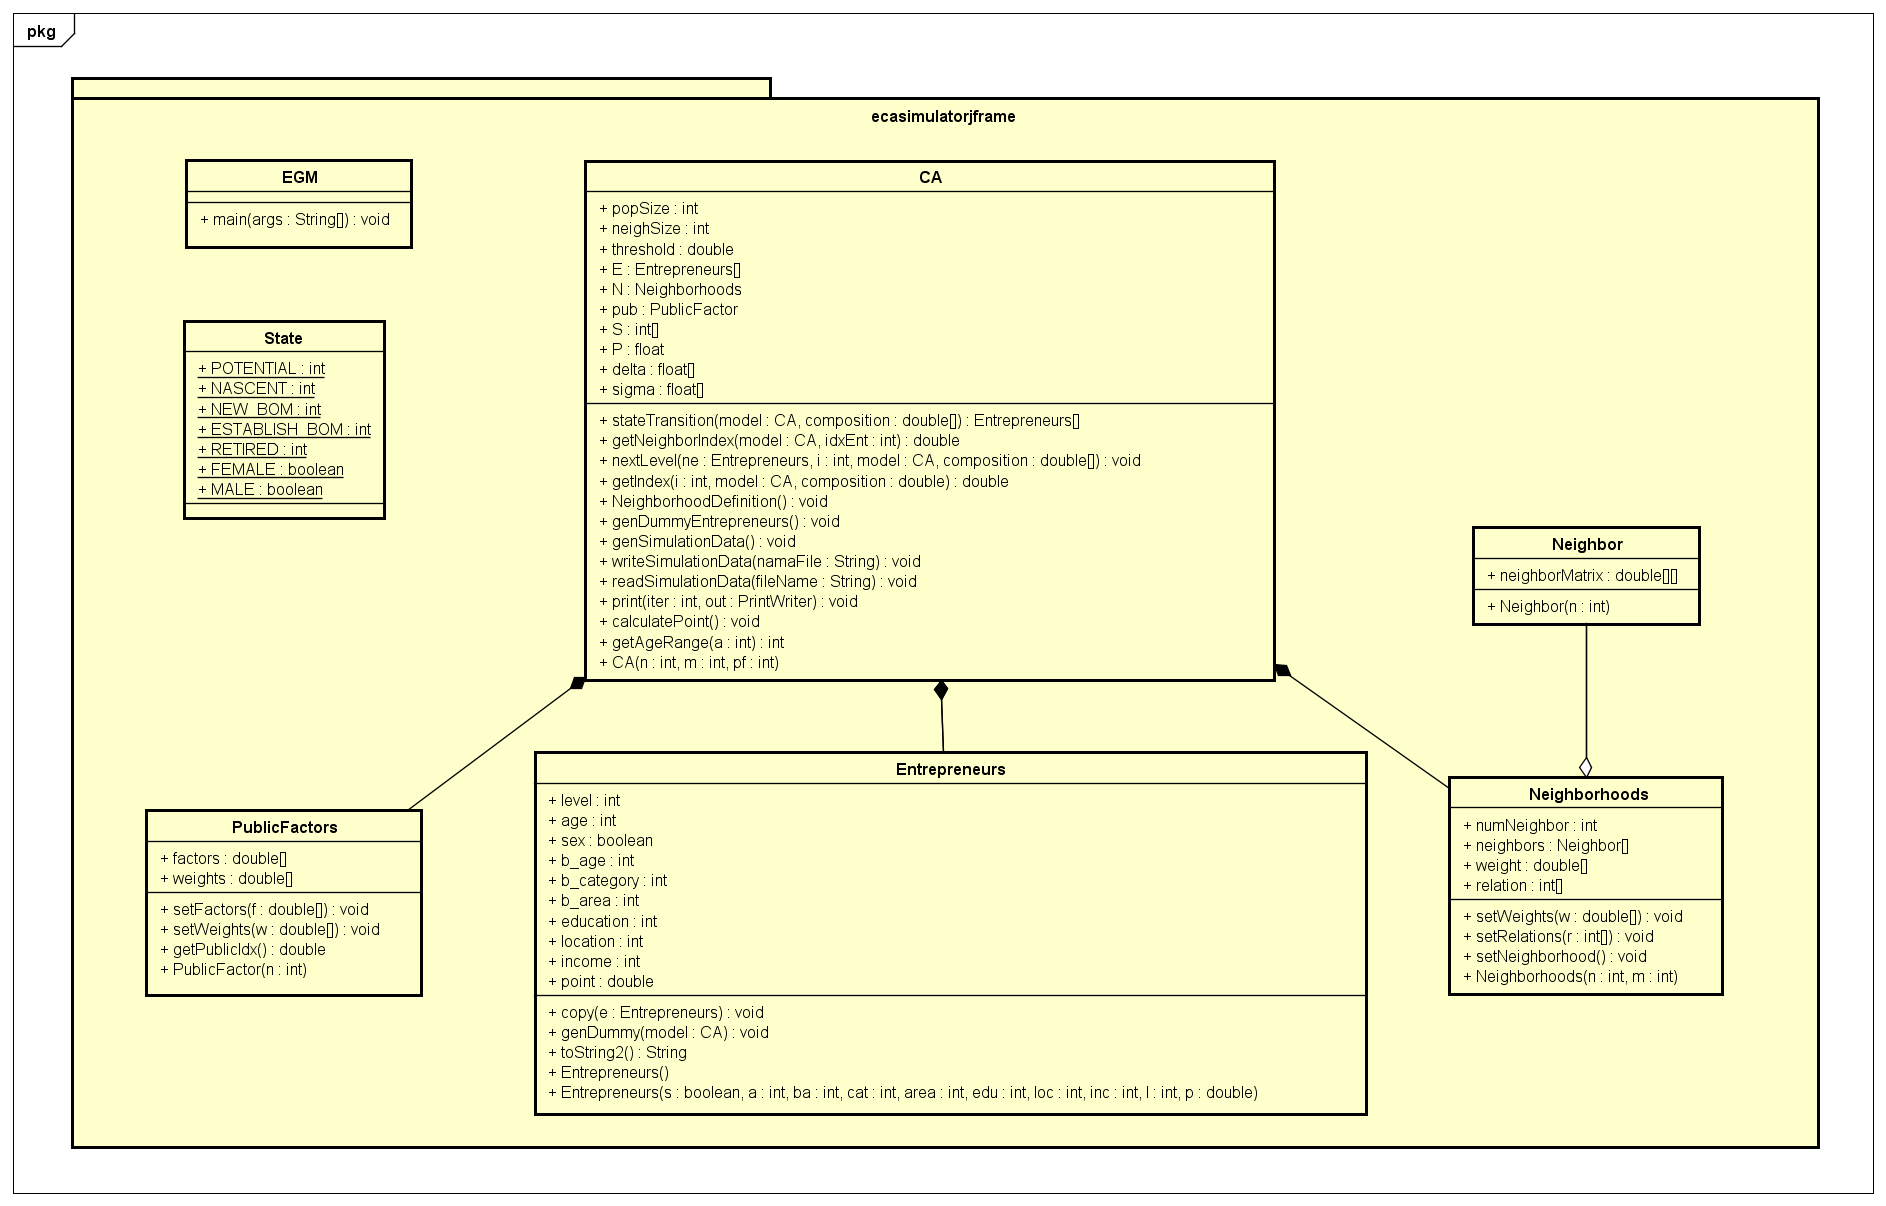
\includegraphics[width=18cm, height=13cm]{diagramKelas0} 
		\caption[Diagram Kelas ECA]{Diagram Kelas ECA} 
		\label{fig:CD1} 
	\end{figure}
	

\subsection{Kelas EGM}
	Kelas EGM merupakan kelas untuk menjalankan perhitungan CIDx, CIDx merupakan angka yang mengindikasikan kemungkinan seorang wirausahawan untuk meneruskan usahanya. Perhitungan CIDx ini menggunakan data dari GEM 2013.
	
\subsection{Kelas CA} 
Kelas CA merupakan kelas yang merepresentasikan \textit{cellular automata}. Untuk \textit{method} \texttt{calculatePoint()} pada diagram kelas \ref{fig:CD1} tidak dituliskan parameternya karena parameternya sangat banyak, maka dari itu akan dijelaskan lebih lanjut pada nomor ke 11. Berikut akan dijelaskan beberapa \textit{method} yang ada di kelas CA :
		\begin{enumerate}
			\item \texttt{public Entrepreneurs[] stateTransition(CA model, double[] composition)}\\
			Merupakan method untuk menentukan perubahan transisi pada seorang wirausaha yang bergantung pada umur dan nilai ambang.\\			Parameter:
			\begin{itemize}
				\item \texttt{model} merupakan objek dari kelas CA.
				\item \texttt{composition} merupakan nilai a,b dan c.
			\end{itemize}
			
			\item \texttt{public double getNeighborIndex(CA model, int idxEnt)}\\
			Merupakan method untuk menghitung nilai dari kondisi ketetanggaan setiap wirausaha.\\
			Parameter:
			\begin{itemize}
				\item \texttt{model} merupakan objek dari kelas CA.
				\item \texttt{idxEnt} merupakan indeks dari wirausaha.
			\end{itemize}
		
			\item \texttt{public void nextLevel(Entrepreneurs ne, int i, CA model, double[] composition)}\\
			Merupakan method untuk menentukan perubahan level usaha dari seorang wirausaha.\\
			Parameter:
			\begin{itemize}
				\item \texttt{ne} merupakan objek dari kelas Entrepreneurs.
				\item \texttt{i} merupakan indeks.
				\item \texttt{model} merupakan objek dari kelas CA.
				\item \texttt{composition} merupakan nilai dari a,b dan c.
			\end{itemize}
			
			\item \texttt{public double getIndex(int i, CA model, double[] composition)}\\
			Merupakan method untuk menghitung CIDx.\\
			Parameter:
			\begin{itemize}
				\item \texttt{i} merupakan indeks.
				\item \texttt{model} merupakan objek dari kelas CA.
				\item \texttt{composition} merupakan nilai dari a,b dan c.
			\end{itemize}
			
			\item \texttt{public void NeighborhoodDefinition()}\\
			Merupakan method untuk mendefinisikan jenis-jenis ketetanggaan seperti lebih dari sama dengan, sama dengan dan lebih kecil sama dengan.\\
			
			\item \texttt{public void genDummyEntrepreneurs()}\\
			Merupakan method untuk membuat data \textit{dummy} wirausaha.
			
			\item \texttt{public void genSimulationData()}\\
			Merupakan method untuk membuat data wirausaha secara \textit{random}.
			
			\item \texttt{public void writeSimulationData(String namaFile)}\\
			Merupakan method untuk menampilkan hasil simulasi ke dalam suatu file.\\
			Parameter:
			\begin{itemize}
				\item \texttt{namaFile} merupakan file tempat hasil simulasi akan ditampilkan.
			\end{itemize}
			
			\item \texttt{public void readSimulationData(String fileName)}\\
			Merupakan method untuk membaca dan memasukkan data file yang akan yang akan disimulasi.\\
			Parameter:
				\begin{itemize}
				\item \texttt{fileName} merupakan file untuk menyimpan hasil simulasi.
			\end{itemize}
			
			\item \texttt{public void print(int iter,PrintWriter out)}\\
			Merupakan method untuk menampilkan jumlah dari masing-masing level wirausaha.\\
			Parameter:
			\begin{itemize}
				\item \texttt{iter} merupakan iterasi per bulan.
				\item \texttt{out} untuk menge-\textit{print} hasil.
			\end{itemize}
			
			\item \texttt{ public void calculatePoint(double[] POAm, double[] POAf, double[] POEf, double[] POEm, double[] POLm, double[] POLf, double[] POIm, double[] POIf, double[] PCAf, double[] PCAm, double[] PCEm, double[] PCEf, double[] PCLm, double[] PCLf, double[] PCIm, double[] PCIf, double[] RMAm, double[] RMAf, double[] RMIm, double[] RMIf)}\\
			Merupakan method untuk menghitung kondisi internal dari seorang wirausaha.\\
			Parameter:
			\begin{itemize}
				\item \texttt{POAm} merupakan kumpulan nilai dari Perceived Opportunities berdasarkan umur (pria).
				\item \texttt{POAf} merupakan kumpulan nilai dari Perceived Opportunities berdasarkan umur (wanita).
				\item \texttt{POEm} merupakan kumpulan nilai dari Perceived Opportunities berdasarkan pendidikan (pria).
				\item \texttt{POEf} merupakan kumpulan nilai dari Perceived Opportunities berdasarkan pendidikan (wanita).
				\item \texttt{POLm} merupakan kumpulan nilai dari Perceived Opportunities berdasarkan lokasi (pria).
				\item \texttt{POLf} merupakan kumpulan nilai dari Perceived Opportunities berdasarkan lokasi (wanita).
				\item \texttt{POIm} merupakan kumpulan nilai dari Perceived Opportunities berdasarkan pendapatan (pria).
				\item \texttt{POIf} merupakan kumpulan nilai dari Perceived Opportunities berdasarkan pendapatan (wanita).
				\item \texttt{PCAm} merupakan kumpulan nilai dari Perceived Capabilities berdasarkan umur (pria).
				\item \texttt{PCAf} merupakan kumpulan nilai dari Perceived Capabilities berdasarkan umur (wanita).
				\item \texttt{PCEm} merupakan kumpulan nilai dari Perceived Capabilities berdasarkan pendidikan (pria).
				\item \texttt{PCEf} merupakan kumpulan nilai dari Perceived Capabilities berdasarkan pendidikan (wanita).
				\item \texttt{PCLm} merupakan kumpulan nilai dari Perceived Capabilities berdasarkan lokasi (pria).
				\item \texttt{PCLf} merupakan kumpulan nilai dari Perceived Capabilities berdasarkan lokasi (wanita).
				\item \texttt{PCIm} merupakan kumpulan nilai dari Perceived Capabilities berdasarkan pendapatan (pria).
				\item \texttt{PCIf} merupakan kumpulan nilai dari Perceived Capabilities berdasarkan pendapatan (wanita).
				\item \texttt{RMAm} merupakan kumpulan nilai dari Role Model berdasarkan umur (pria).
				\item \texttt{RMAf} merupakan kumpulan nilai dari Role Model berdasarkan umur (wanita).
				\item \texttt{RMIm} merupakan kumpulan nilai dari Role Model berdasarkan pendapatan (pria).
				\item \texttt{RMIf} merupakan kumpulan nilai dari Role Model berdasarkan pendapatan (wanita).
			\end{itemize}
			
			\item \texttt{public int getAgeRange(int a)}\\
			Merupakan method untuk membedakan rentang usia yang telah ditentukan oleh GEM 2013.\cite{GEM2013}\\
			Parameter:
			\begin{itemize}
				\item \texttt{a} merupakan umur wirausaha.
			\end{itemize}
		\end{enumerate}
		
\subsection{Kelas Entrepreneurs} 
	Kelas Entrepreneur merupakan kelas untuk merepresentasikan individu wirausahawan.
\subsection{Kelas Neighbor}
	Kelas Neighbor merupakan kelas untuk merepresentasikan ketetanggaan untuk satu aspek tertentu. Setiap aspeknya didefinisikan sebagai satu neighbor yang berupa adjacency matrix.
\subsection{Kelas Neighborhood}
	Kelas Neighborhood merupakan kelas untuk merepresentasikan himpunan ketetanggaan yang tersusun atas sejumlah ketetanggaan.
\subsection{Kelas Public Factor}
	Kelas PublicFactor merupakan kelas untuk merepresentasikan faktok publik.
\subsection{Kelas State}
	Kelas State merupakan kelas untuk memberi nilai untuk setiap level wirausaha.


